\documentclass[11pt]{article}
\usepackage[utf8]{inputenc}
\usepackage[T1]{fontenc}
\usepackage{amsmath}
\usepackage{amsfonts}
\usepackage{amssymb}
\usepackage[version=4]{mhchem}
\usepackage{stmaryrd}
\usepackage{graphicx}
\usepackage[export]{adjustbox}
\graphicspath{ {./images/} }

\begin{document}
\section*{Reading}
Internal Rate of Return

The computation of traditional investment returns is not easy, but it is far easier than the computation of returns for some alternative investments. A main challenge with the analysis of some alternative investments is the lack of regularly observable market prices. Some alternative investments, such as private equity and private real estate, are analyzed using an internal rate of return approach. This approach has numerous potential complications and shortcomings. With the advantage of regular market prices, traditional investment analysis usually computes return as the change in price, net of fees, plus cash flows received (such as dividend or interest payments), divided by the initial price:


\begin{equation*}
\text { Rate of Return }=\text { (Change in Price }+ \text { Cash Flows }) / \text { Initial Price } \tag{1}
\end{equation*}


However, complications arise when prices cannot be regularly observed or when cash flows are received during the interim period, between the starting date and the ending date of the return observation. A major complexity related to these interim cash flows is that it is unclear how much return could be earned through their reinvestment. It is usually assumed that the intervening cash flows are reinvested in the same underlying investment, but this requires an interim price of that asset at the same time as the cash flows become available for reinvestment.

Since prices can be observed at least on a daily basis for most traditional investments, daily returns are easily computed from daily prices and daily cash flows. Returns over time periods in excess of one day with intervening cash flows can be computed as the accumulation of the daily returns within the time period. In other words, returns for longer time periods are formed from the daily returns of the days within the time period. Returns over time periods shorter than one day do not tend to have intervening cash flows, since dividends and interest payments are usually made on an end-of-day basis.

Despite challenges faced with various compounding assumptions and intervening cash flows, calculating the returns of most traditional investments is relatively straightforward when daily prices are available. However, return computations for investments that cannot be accurately valued each day generate challenges that are a primary topic of this session. For example, securities that are not publicly traded, such as private equity, do not have unambiguous daily valuations that can be used to compute daily returns. This section explains the application of the internal rate of return method to alternative investments and details the potential difficulties with interpreting and comparing internal rates of return.

\section*{Defining the IRR}
The internal rate of return (IRR) can be defined as the discount rate that equates the present value of the costs (cash outflows) of an investment with the present value of the benefits (cash inflows) from the investment. Using the terminology and methods of finance, the IRR is the discount rate that makes the net present value (NPV) of an investment equal to zero.

Let $C F_{0}$ be the cash flow or a valuation related to the start of an investment (i.e., at time 0 ). $C F_{0}$ might be the cost of an investment in real estate, or in the case of private equity, $C F_{0}$ might be the initial investment required to obtain the investment or meet the fund's first or only capital infusion; $C F_{1}$ through $C F_{T-1}$ are the actual or projected cash inflows if positive and cash outflows if negative, generated or required by the underlying investment. Positive cash flows are distributions from the investment to the investor, and negative cash flows are capital calls in which an additional capital contribution is required of each investor to the investment.

A $C F_{T}$ may be the final cash flow when the investment terminates, the final cash flow received from selling or otherwise disposing of the investment, or a residual valuation, meaning some appraisal of the value of the remaining cash flows related to the investment. In the case of an appraised valuation of $C F_{T}$, the valuation should be designed to represent opinions with regard to the amount of cash that would be received from selling all remaining rights to the investment. The values are denoted here with the variable $C F$, which usually stands for cash flows, even though they may be hypothetical values or appraised values for the investments rather than actual cash flows.

Given all cash flows and/or valuations from period 0 to period $T$, the IRR is the interest rate that sets the left-hand side of Equation 2 to zero:


\begin{equation*}
C F_{0}+\frac{C F_{1}}{(1+\mathrm{IRR})^{1}}+\frac{C F_{2}}{(1+\mathrm{IRR})^{2}}+\frac{C F_{3}}{(1+\mathrm{IRR})^{3}}+\ldots+\frac{C F_{T}}{(1+\mathrm{IRR})^{T}}=0 \tag{2}
\end{equation*}


Another view of the IRR is that it is the interest rate that a bank would have to offer on an account to allow an investor to replicate the cash flows of the investment. In other words, if an investor deposited $C F_{t}$ in a bank account at time $t$ for each $C F_{t}<0$ and withdrew $C F_{t}$ from the bank account when $C F_{t}>0$, and if the bank's interest rate on the account was IRR, then the bank account would have a zero balance after the last cash flow was deposited or withdrawn $\left(C F_{T}\right)$.

\section*{Computing the IRR}
In some simplified cases, such as investments that last only a few periods or investments in which most of the cash flows are identical (i.e., annuities), the IRR may be solved algebraically with a closed-form solution. In cases involving several different cash flows, the solution generally relies on a trial-and-error search performed by an advanced financial calculator or computer.

A simplified example to illustrate the trial-and-error method involves an investment that costs $\$ 250$ million and lasts three years, generating cash inflows of $\$ 150$ million, $\$ 100$ million, and $\$ 80$ million in years 1,2 , and 3 , respectively. The IRR is found as that interest rate that solves the following equation:


\begin{equation*}
-\$ 250 \mathrm{M}+\frac{\$ 150 \mathrm{M}}{(1+\mathrm{IRR})^{1}}+\frac{\$ 100 \mathrm{M}}{(1+\mathrm{IRR})^{2}}+\frac{\$ 80 \mathrm{M}}{(1+\mathrm{IRR})^{3}}=0 \tag{3}
\end{equation*}


The trial-and-error process selects an initial guess for IRR, such as 10\%, and then searches for the correct answer: the IRR that sets the left-hand side of Equation 3 to zero. Inserting IRR $=0.10(10 \%)$ into Equation 3 generates a present value of inflows equal to $\$ 279.11$ million and a value to the entire left-hand side of $\$ 29.11$ million. The objective is to have the value of the left-hand side of the equation equal to zero. In the case of this investment, a higher discount rate will generate a lower net value. If the next guess is an interest rate of $15 \%$, the value of the left-hand side of the equation declines to $\$ 8.65$ million. The process continues with as much precision as required. The IRR of this investment is $17.33 \%$ carried to the nearest basis point.

Advanced calculators and computer spreadsheets perform the trial-and-error process automatically. This solution of $17.33 \%$ for the IRR can be found on most financial calculators by inserting the cash flows (using cash flow mode) and requesting the computation of the IRR or in a spreadsheet with a function designed to compute IRR.

In this example, the trial-and-error process for finding the IRR works well because any increase in the discount rate lowers the present value of the cash inflows, and any decrease in the discount rate raises the present value of the inflows. The solution to the IRR problem is illustrated in the next exhibit, The Solution to IRR in a Simplified Investment. For example, on a Texas Instrument BA II Plus calculator the keystrokes can be: [on/off], CF, $2^{\text {nd }}$, [CE/C], 250, [+/-], enter $\downarrow, 150$, enter, $\downarrow \downarrow, 100$, enter, $\downarrow \downarrow, 80$, enter, IRR, CPT. The IRR is 17.33415 .

Because the IRR is the discount rate that sets the NPV of the investment to zero, the IRR is represented by the point at where the NPV curve crosses through the horizontal axis. This occurs between $17 \%$ and $18 \%$ on the figure, which corresponds to the previous solution of $17.33 \%$. There is only one solution, and it is quite easily found. If a bank offered an interest rate of $17.33 \%$, then an investor could deposit $\$ 250$ million and withdraw $\$ 150$ million, $\$ 100$ million, and $\$ 80$ million after one, two, and three years, respectively; and the final account balance would be $\$ 0$, ignoring rounding errors.

\begin{center}
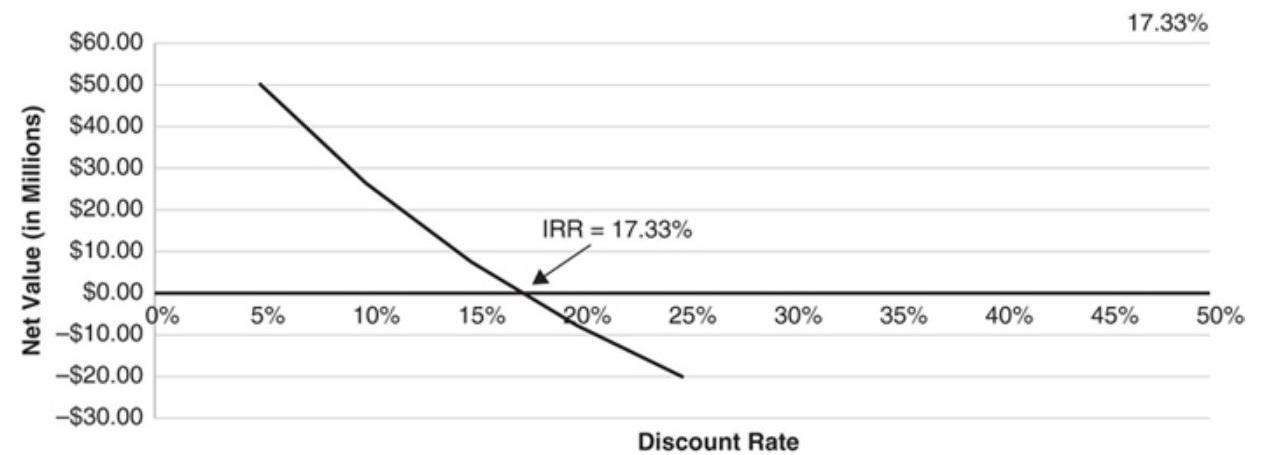
\includegraphics[max width=\textwidth]{2024_04_10_52a8c38b9d0ded03b349g-3}
\end{center}

The Solution to IRR in a Simplified Investment

\section*{IRR Measurement Intervals}
The primary reason for using the IRR approach to calculate returns is that illiquidity of the underlying asset prevents observation of highly reliable and regular valuations, such as daily market prices. This section discusses types of IRRs differentiated by the time periods over which cash flows and net asset values are estimated. Subsequent sections detail modified IRR and, in Level 2, the public equivalent IRR method.

One distinction between IRR computations is whether the cash flows are realized (observed), expected (projected), or appraised (e.g., a net asset value). Another distinction is whether the underlying investment is a single asset or a fund. Finally, IRRs are distinguished by the time interval over which the IRR is estimated relative to the inception and termination of the underlying asset. Technically, all IRR computations are point-to-point computations. Although the terms that follow are not uniformly defined in practice, they are useful for our purposes.

A lifetime IRR contains all of the cash flows, realized or anticipated, occurring over the investment's entire life, from its beginning to its termination. An interim IRR is a computation of IRR based on cash flows prior to the investment's termination. The key to an interim IRR is that generally the final cash flow at time $T$ in the analysis would not be the termination of the investment; thus, $C F_{T}$ is an estimated value rather than a realized cash flow. A since-inception IRR is an interim IRR that starts with the underlying investment's initial cash flow (inception date). Also, a since-inception IRR is commonly used as a measure of fund performance rather than the performance of an individual investment.


\end{document}